\chapter{Jets} \label{ch:jets}

A jet is a collimated spray of stable particles measurable in the detector,
which arises from the production of a quark or gluon in the scattering process.
Due to QCD confinement, the quarks and gluons themselves can never be observed,
so jets serve as a kind of observable proxy for these more fundamental particles.
However, there is not a simple one-to-one correspondence between each jet measured in an event and a quark or gluon in the hard scattering process.
Due to the complex nature of proton-proton collisions, as well as the fundamental probabilistic nature of quantum mechanics,
the partonic source for a given jet can never be specified exactly.
Likewise, when performing theoretical calculations, the number and property of jets that arise from a given parton produced in the hard scattering
can only be specified probabilistically.
Section~\ref{sec:jet_collisions} will explain the many different parts of a proton-proton collision that contribute to jet production.

Furthermore, the number and properties of jets measured in a single event will depend on the choice of jet reconstruction algorithm.
In order for experimentalists to test the predictions of theory, it's important for standard jet definitions to be decided upon.
While there is no one theoretically correct choice of jet definition, there are certain properties of jet algorithms
that make them more or less desirable.
The different kinds of jet algorithms and their properties will be discussed in section~\ref{sec:jet_clustering}

Section~\ref{sec:jet_substructure} will discuss jet substructure, which are the internal properties of jets.
And section~\ref{sec:jet_reconstruction} will explain the process of jet reconstruction and calibration in ATLAS.

\section{The proton-proton collision environment}\label{sec:jet_collisions}

As discussed in~\ref{subsec:qcd_pdfs}, the goal of proton-proton collision experiments is to understand the interactions
between fundamental particles, but due to QCD confinement it is impossible to simply collide the individual partons of interest.
Instead, complicated bound states of quarks and gluons are collided,
with the goal of measuring the processes that occur when constituent partons collide with each other.
As a result, proton-proton collision events create a very messy environment from which the hard-scatter process
has to be deduced.

QCD confinement also has the consequence that the final state quarks and gluons created in LHC collisions
can never be directly detected.
Instead, collimated sprays of hadrons, called jets, must be measured in order to attempt to reconstruct the
hard scattering process that gave rise to them.

Figure~\ref{fig:jet_tth_diagram} illustrates a typical proton-proton collision event,
in which two gluons annihilate to generate a Higgs boson along with a top-antitop quark pair.
Even though this is not a dijet or multijet production event,
it is useful for understanding all the parts of a proton-proton collision that must be considered when calculating the
predicted rates of multijet production.

\begin{figure}[h!]
    \centering
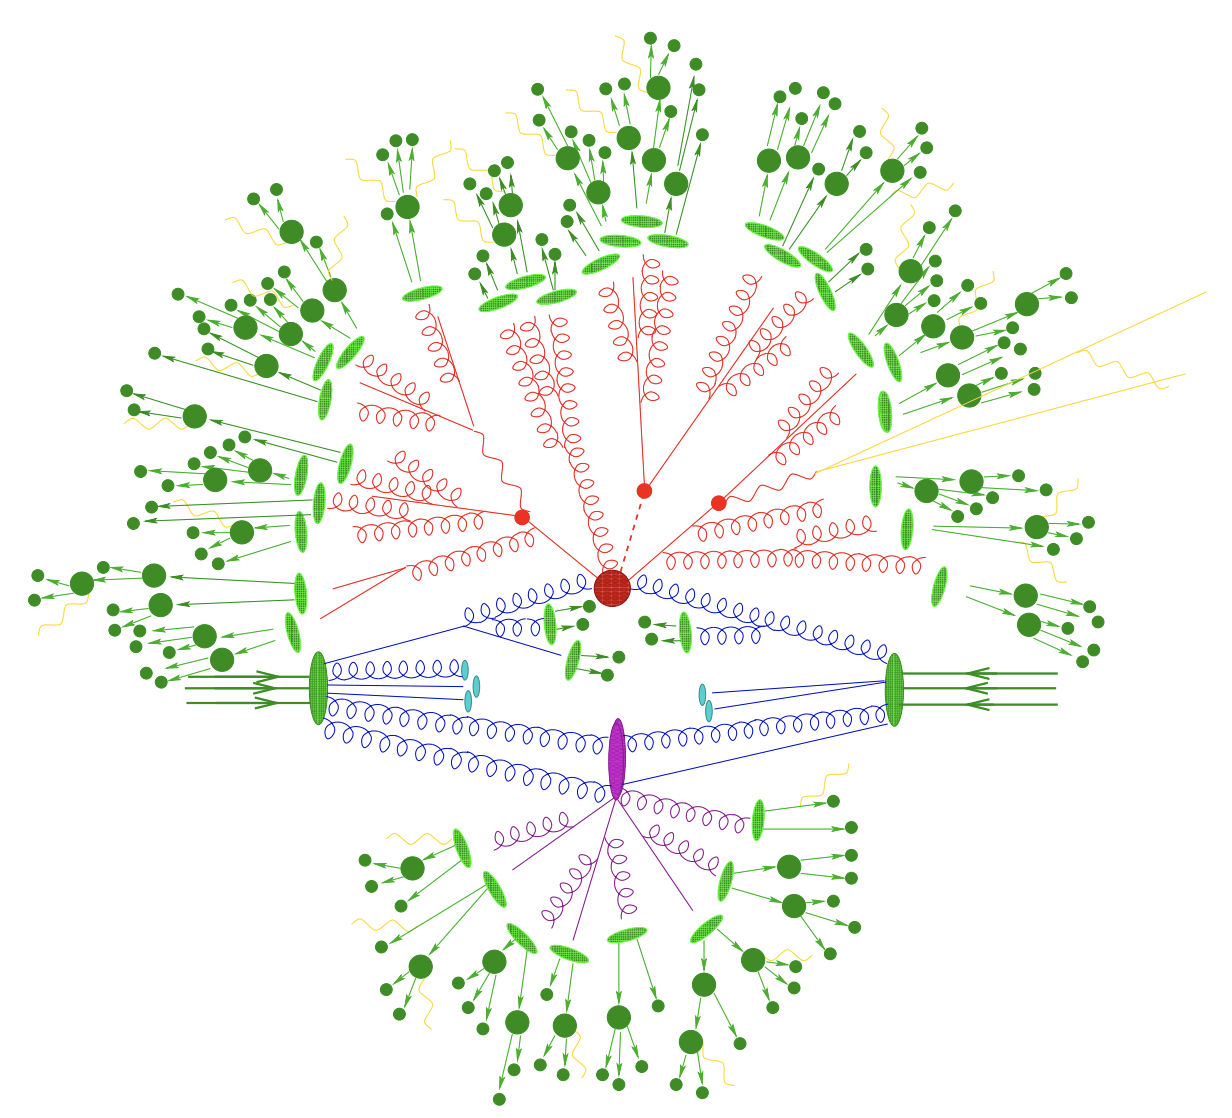
\includegraphics[width=0.6\linewidth]{jet_tth_diagram}
\caption{Diagram of a proton-proton collision event in which the hard scatter process is $t\bar{t}H$ production.
Illustrated are the initial state radiation, underlying event, hard-scatter process, final state parton shower,
fragmentation, hadron decays, and final state QED radiation.}
\label{fig:jet_tth_diagram}
\end{figure}\cite{sherpa-2004}

The incoming protons are illustrated by green blob with three incoming arrows to represent the constituent quarks.
The initial state parton showering, governed by QCD, is shown in blue.
The hard scatter process, in which two gluons annihilate to produce a Higgs boson and top-antitop pair is represented
by the large red circle.
Quarks and gluons from the incoming proton that do not participate in the hard scatter process can nonetheless interact
with each other, creating a so-called underlying event, shown in purple.
The Higgs decays to a quark-antiquark pair, shown in red, and all of the strongly-interacting final state quarks
and gluons undergo final state parton showering, also in red.
Once the final state parton shower particles reach a low enough energy, they hadronize, a non-perturbative process
indicated by the light green blobs.
The resulting hadrons then decay through various decay chains, shown in dark green.
Photon radiation, governed by QED, can occur at any of these stages, and is shown in yellow.

The final measured objects in the detector are the jets.
But every process leading up to the final state is quantum mechanical,
meaning that interference terms between the various processes lead to a fundamental and unresolvable ambiguity in the source of a given jet.

An event with 3 high-$pT$ jets could be explained by a $2\rightarrow3$ hard-scattering process,
or a $2\rightarrow2$ hard scattering process, with an additional jet arising from ISR or FSR, the underlying event,
or even from a hadronic decay.
All of these processes must be taken into account when calculating the rate of 3-jet events,
each contributing its own source of uncertainty.
The final rate calculation combines the perturbative QCD calculations for the matrix elements and parton showering
with empirically measured probability distributions for the non-perturbative parts of the collision,
including soft gluon emission, long-distance couplings, hadronization, and multi-parton interactions (MPI). 
As the number of jets in the final state increases, so does the complexity and uncertainty when calculating event rates.

Monte Carlo (MC) generators attempt to account for all of these effects to calculate the rate of multijet events at the LHC .
However, the MC estimates have very large uncertainties, for the reasons given above.
As a result, data driven estimation methods are used for determining the background rate of multijet events.

\section{Clustering Algorithms}\label{sec:jet_clustering}

In order to measure jets in an event, a decision has to be made on the type of jet reconstruction algorithm to use.
The observable result of a collision event can consists of many clusters of stable particles or calorimeter hits.
Exactly which particles to cluster together is highly non-trivial, and developing the algorithms to make these decisions
is an active area of research in particle physics.

The 1990 Snowmass accord defined a set of criteria which should be met by any jet algorithm.
The criteria for a developing a jet reconstruction algorithm are:

\begin{enumerate}
    \item Simple to implement in an experimental analysis
    \item Simple to implement in the theoretical calculation
    \item Defined at any order in perturbation theory
    \item Yields finite cross sections at any order of perturbation theory
    \item Yields a cross section that is relatively insensitive to hadronization
\end{enumerate}\cite{jet-jetography,jet-snowmass}

Jet reconstruction algorithms that meet all of these criteria allow experimentalists to test theoretical prediction,
because both the theoretical calculations and experimental analysis can use the same jet definition.
Jet algorithms are defined as acting on abstract "objects".
The last Snowmass criteria ensures that in theoretical calculations,
jet algorithms can be applied at either the parton-level or hadron level.
In either case, the object which the algorithm acts on will be a particle.
Jet algorithms can also be applied by experimentalists to reconstruct jets from either simulated or real calorimeter hits.
In this case, the object which the algorithm acts on is a cluster of calorimeter hits.

Historically, there have been two major types of jet algorithms used in particle physics experiments:
cone-based algorithms and sequential recombination algorithms.
Cone-based algorithms, which were developed first, aim to cluster jets in $\eta-\phi$ space.
They are fast and easy to implement, and produce jets with regular boundaries in $\eta-\phi$ space,
but have many theoretical and practical downsides compared to sequential recombination algorithms.
They typically use the highest-transverse-momentum (hardest) object in the event as a seed for a jet cone,
then define a cone around that seed as the leading jet,
before moving on to the next-hardest object.
Cone-based algorithms have the advantage of producing regularly-shaped jet boundaries,
which can simplify theoretical calculations and make experimental calibration easier~\cite{jet-cone-algo}.
However, cone-based algorithms typically collinear safety,
which are properties that need to be satisfied to meet the Snowmass criteria.

\subsection{IRC Safety}\label{subsec:jet_irc_safety}

Jet algorithms should ideally possess infrared and collinear (IRC) safety.
This means that their results should not change due to soft gluon emissions or near-collinear emissions
during either the parton shower or hadronization process.
IRC safety is important because soft and collinear emissions are extremely common in QCD,
occur randomly, are hard to predict, and can lead to divergences in perturbative calculations if the algorithm is IRC-unsafe.\cite{jet-jetography}

\subsubsection{Collinear safety}

A collinear-safe algorithm is insensitive to near-collinear emissions that occur during parton showering or hadron decays.
Cone-based algorithms are collinearly unsafe because they seed jets with the hardest object in the event,
which is very likely to change if there is a near-collinear emission.

In figure~\ref{fig:jet_collinear_safety}, for the collinear-unsafe cone-based algorithm,
the hardest object in the event changes depending on whether the radiated gluon is reabsorbed or emitted nearly collinear to the original quark.
Thus, the resulting seed will change, yielding different jet results.
The loop diagram and collinear emission diagram both lead to divergences in the theoretical cross-section.
In a collinear-safe algorithm, the two divergences would cancel out because both amplitudes must be added to calculate the rate
of the single jet being produced.
But in a collinear-unsafe algorithm, the two divergences do not cancel out, so perturbation cross-sections are not finite.

\begin{figure}[h!]
    \centering
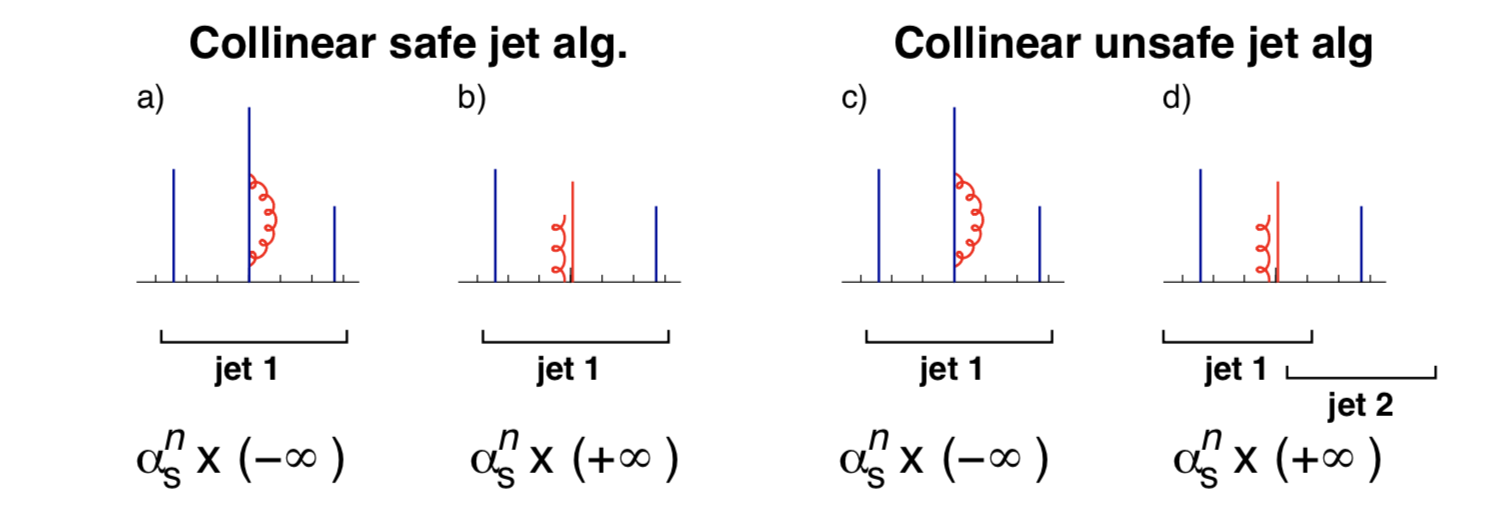
\includegraphics[width=0.9\linewidth]{jet_collinear_safety}
\caption{Illustration comparing the results of collinear-safe (left) and collinear-unsafe (right) jet clustering algorithms.
The emission of a near-collinear gluon changes the number of jets in the event, and results in diverges in theoretical calculations.
The x-axis represents rapidity, and y-axis represents transverse momentum.}
\label{fig:jet_collinear_safety}
\end{figure}\cite{jet-jetography}

\subsubsection{Infrared safety}

A related concept is that of infrared safety.
Jet algorithms should insensitive to soft gluon emissions.
These emissions are extremely common during parton showering, and since they occur in the non-perturbative regime of QCD,
very hard to accurately predict.

Figure~\ref{fig:jet_ir_safety} illustrates the result of an infrared-unsafe algorithm.
A W boson decays to a quark-antiquark pair, which should result in two hard jets.
Diagrams (b) and (c) each lead to IR divergences, which would cancel if the algorithm is infrared-safe.
But for an infrared-unsafe algorithm, diagram (c) leads to a different number of jets from diagram (b),
so the divergences do not cancel.

\begin{figure}[h!]
    \centering
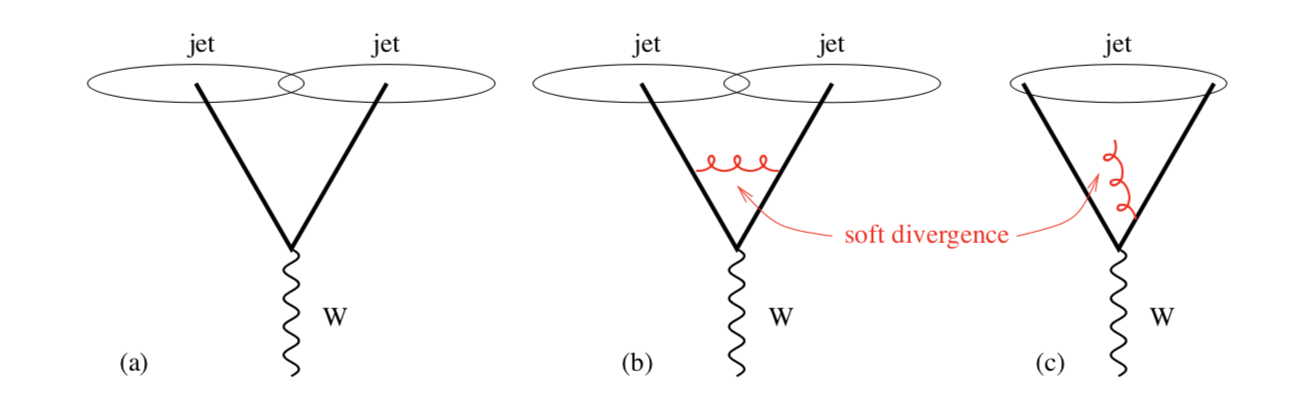
\includegraphics[width=0.9\linewidth]{jet_ir_safety}
\caption{Illustration of infrared unsafety.
In an event with a W boson decaying to two hard partons, the emission of a soft gluon can change the result of an infrared-unsafe algorithm.}
\label{fig:jet_ir_safety}
\end{figure}\cite{jet-jetography}

\subsection{Sequential recombination algorithms}\label{subec:jet_seq_recombination}

Sequential recombination algorithms are the most commonly used jet algorithms in ATLAS today.
Instead of clustering in $\eta-\phi$ space, they cluster in transverse momentum space.
The resulting jets have irregular boundaries, which adapt to soft radiation.
Sequential recombination algorithms are generally slower to run,
but have become more popular since the invention of the FastJet\cite{jet-fastjet} algorithm.
Sequential recombination algorithms are IRC safe.

All sequential recombination algorithms start by defining a distance measure:

\begin{align}\label{eq:jet_distance}
    d_{ij} = min\left(k_{Ti}^{2p}, k_{Tj}^{2p}\right)\frac{\Delta_{ij}}{R^2} \\
    d_{iB} = k_{Ti}^{2p}
\end{align}

Where the indices $i$ and $j$ are used for two objects under consideration,
$d_{ij}$ is the distance between those two objects, $k_T$ is the transverse momentum,
$\Delta_{ij}^2 \equiv (\eta_i-\eta_j)^2 + (\phi_i-\phi_j)^2$ is the distance-squared in $\eta-\phi$ space,
and $p$ and $R$ are two parameters that control the behavior of the algorithm.
The object-beam distance, $d_{iB}$ is also used by the algorithms, and is defined for each object individually rather than for pairs of objects.

The choice of $R^2$ roughly controls the area of the resulting jets.
It is often referred to as a radius parameter, but the jets that result from these algorithms have irregular shapes,
so this term is used loosely.

The choice of $p$ determines the class of sequential recombination algorithms, each of which has different properties.

All sequential reclustering algorithms use these distance measures in the following way:

\begin{enumerate}
    \item Calculate $d_{ij}$ over all pairs of objects, and $d_i$ for each object individually
    \item If the minimum of the set $\{d_{ij}, d_i\}$ is one of the $d_{ij}$'s:
        \subitem Sum the four vectors of objects $i$ and $j$
        \subitem Add the resultant four-vector to the list of objects, and remove the four vectors for objects $i$ and $j$
        \subitem Go to Step 1
    \item Else if the minimum of the set $\{d_{ij}, d_i\}$ is one of the $d_i$'s:
        \subitem Call the object $i$ a jet
        \subitem Remove the object $i$ from the list of objects
        \subitem Go to Step 1
\end{enumerate}

An inclusive clustering algorithm stops when all objects have been clustered into a jet.
An exclusive algorithm stops when a pre-defined number of jets have been clustered.\cite{jet-algo-review}

The Cambridge-Aachen (C/A) algorithm has $p=0$, and so does not directly use the transverse momentum of the jets.
Instead the distance measure is purely in terms of pseudorapidity and azimuthal angle,
so objects are clustered based on how close together they are in this radial distance measure.
The boundaries of resulting jets are sensitive to random fluctuations of soft objects,
such as those from pileup and the underlying event.

The $k_T$ algorithm has $p=1$, and so starts by clustering objects which are both spatially close together and have low momentum.
Like with the C/A algorithm, the resulting jets are sensitive to random flucutations in soft objects from pileup and the underlying event.

In the anti-$k_T$ algorithm, the objects which are closest together and hardest are clustered together first.
The resulting jet shapes are insensitive to the details of the soft radiation.
So the impact of pileup and the underlying event on jet momentum resolution is smallest for the anti-$k_T$ algorithm\cite{jet-antikt-algo}.

A comparison of the different jet clustering algorithms can be seen in figure~\ref{fig:jet_algo_compare}.
The same parton-level simulated event data was input into four different jet clustering algorithms.
Random soft particles were also added to the parton-level event data.
The resulting jets are plotted in $y-\phi$ space, with colors labelling the different jets, and the height of each bar
indicating the transverse momentum in that region.
For the $k_T$ and $C/A$ algorithms, the jet boundaries are highly irregular, and depend strongly on the details of the random soft particles.\cite{jet-antikt-algo}

\begin{figure}[h!]
    \centering
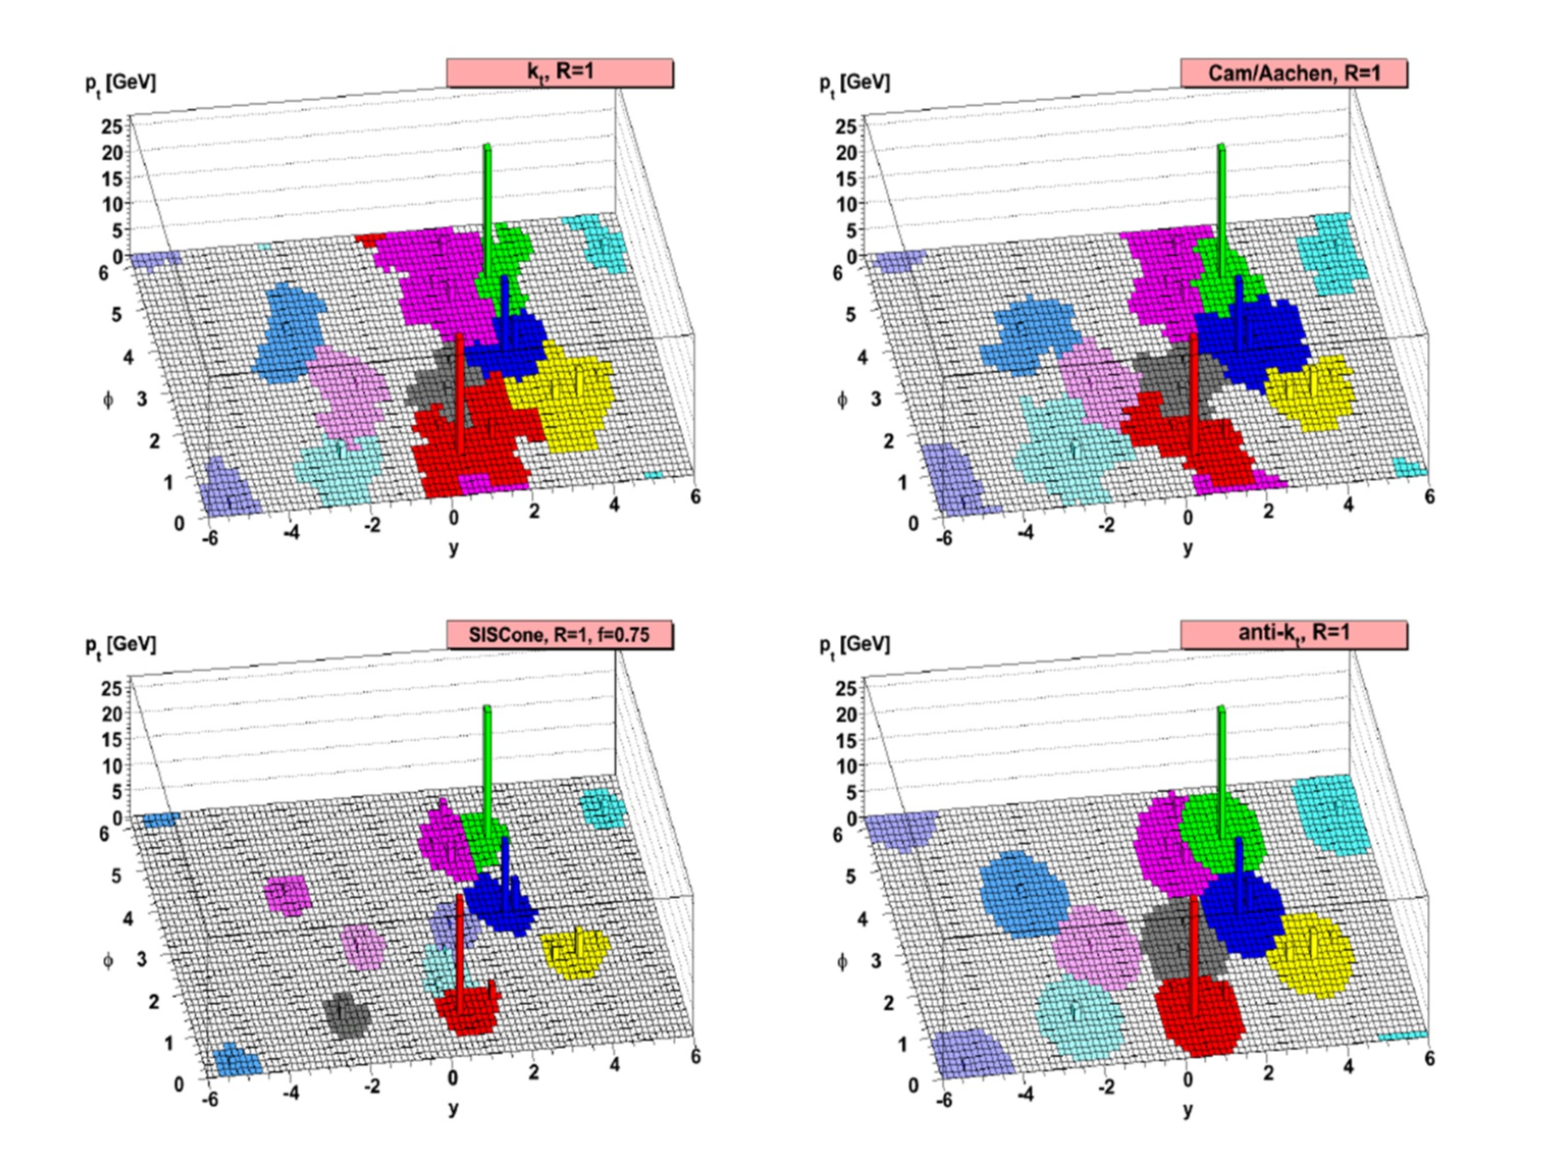
\includegraphics[width=0.9\linewidth]{jet_algo_compare}
\caption{Results of running four different jet clustering algorithm on the same set of parton-level simulated event data.
SISCone (lower-left) is a cone-based algorithm, while the other three are sequential recombination algorithms defined
by different values of $p$.}
\label{fig:jet_algo_compare}
\end{figure}\cite{jet-antikt-algo}

\section{Boosted objects}\label{sec:jet_substructure}

As the center-of-mass energy of collisions increases, it becomes increasingly important to study the internal structure
of jets, in addition to the kinematic properties of jets within events.
The decay products of hadronically-decaying heavy objects, such as W or Higgs bosons,
become harder to resolve into separate jets as the momentum of the original object increases.
Recently, a large number of jet substructure observables have been developed, and an entire subfield has emerged
dedicated to the study of the internal properties of jets.

For a two-pronged decay, for example $W \rightarrow q\bar{q}$, the angular separation between the decay products is given by:

\begin{equation}\label{eq:jet_boosted_sep}
    \Delta R = \frac{p_{T}}{2m}
\end{equation}

Where $p_T$ is the transverse momentum of the $W$, and $m$ is the $W$ mass.
For $W$ bosons with $p_T \gg m$, jets with radius parameter $R = 0.4$ will no longer resolve the decay products into separate jets,
but instead will contain the all decay products of the $W$ into a single jet.

Figure~\ref{fig:jet_radial_sep} illustrates the boosting effect for the simulated decay $Z'\rightarrow t\bar{t}$,
where the $Z'$ represents a new heavy resonance.
Since $m_{Z'} \gg m_{t}$, the top quarks are highly boosted, so their decay products cannot be resolved by jets with $R=0.4$.

On the other hand, jets with $R = 1.0$ will capture all decay products with high efficiency,
so the substructure of $R=1.0$ jets can potentially be used to reconstruct these boosted tops.

\begin{figure}[h!]
    \centering
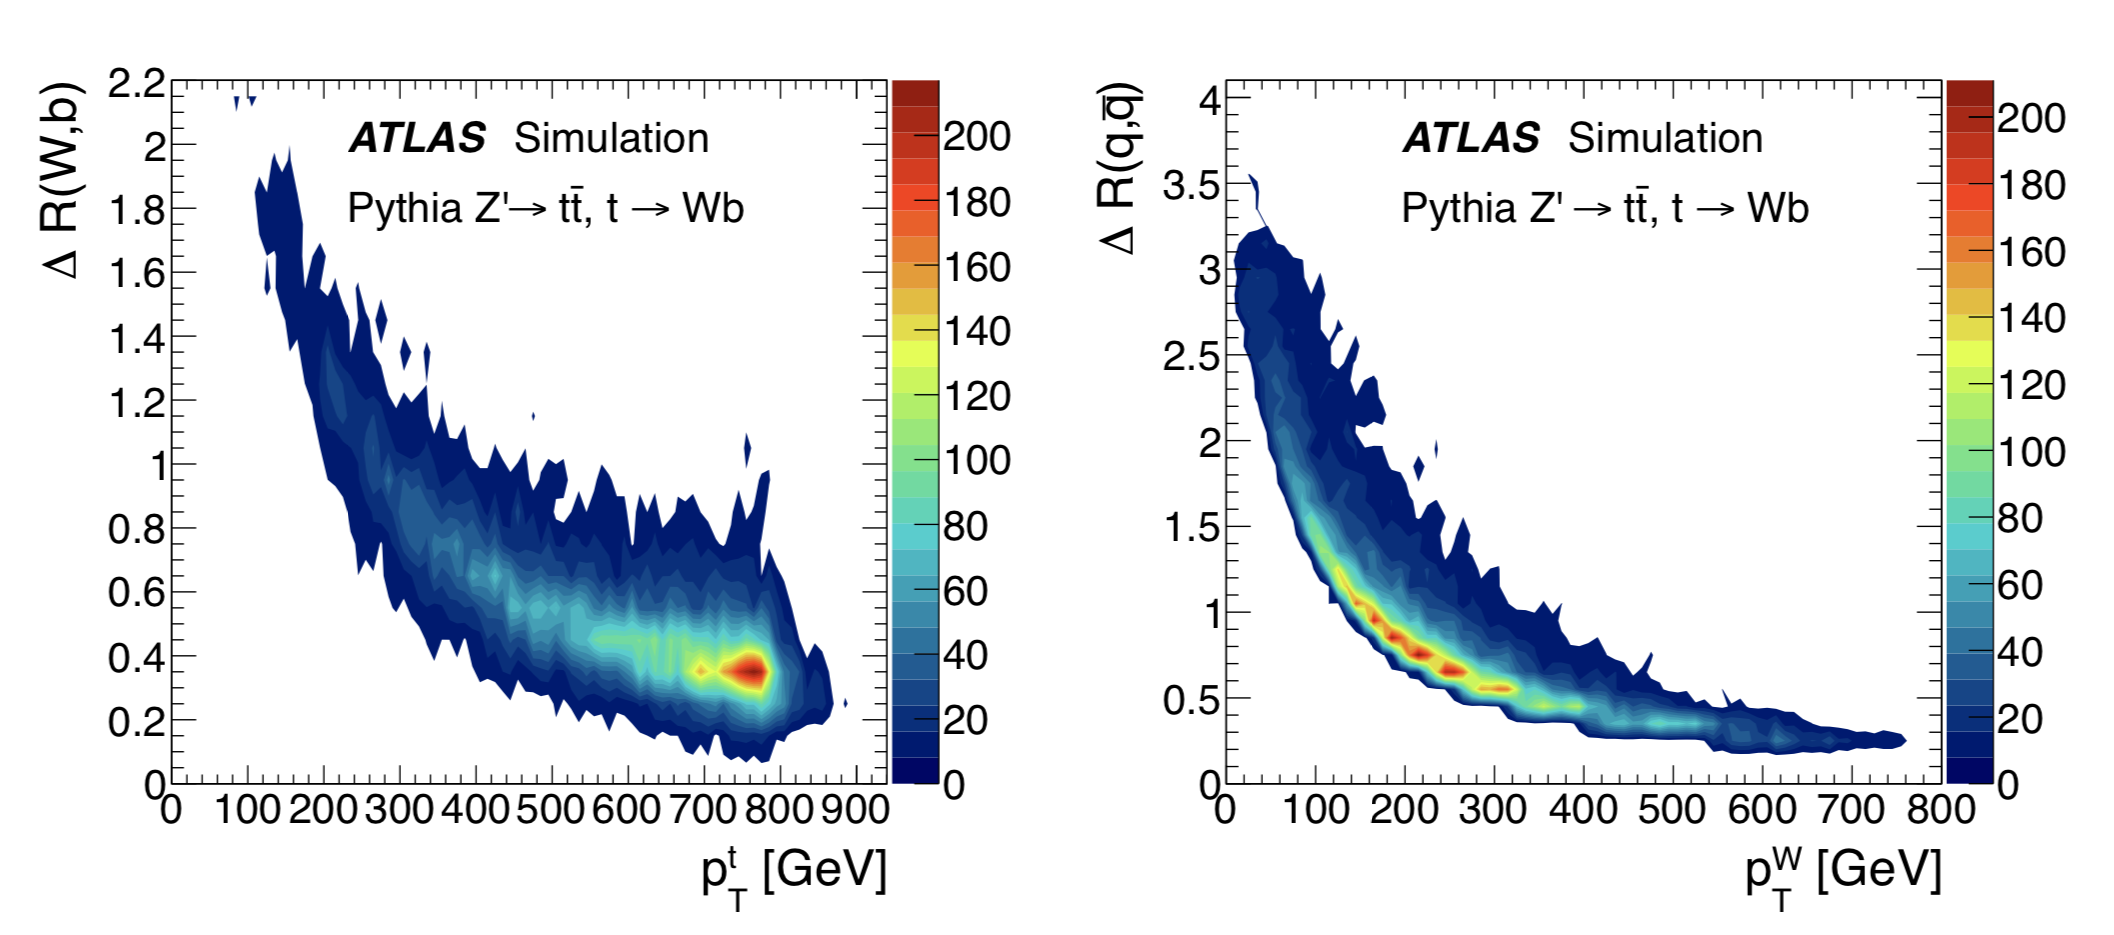
\includegraphics[width=0.9\linewidth]{jet_radial_sep}
\caption{Radial separation between top decay products vs. top-quark $p_T$ for top quarks produced from a theoretical heavy resonance, $Z'$}
\label{fig:jet_radial_sep}
\end{figure}

When dealing with boosted objects, larger radius parameters are often used, in order to increase the probability
of capturing the full decay products of a boosted object.
Jets with large radius parameters, typically $R=1.0$ or $R=1.2$ are referred to as fat jets.

\subsection{Jet Mass}\label{subsec:jet_mass}

\subsubsection{Jet mass origin}

The earliest-developed, and most straightforward jet substructure observable is mass.
The mass of a jet is calculated from the four-vectors of its constituent objects:

\begin{equation}\label{eq:jet_mass}
    m^2 = \left(\sum E_i\right)^2 - \left(\sum \vec{p}_i \right)^2
\end{equation}

For a jet that contains the collimated decay products of an individual boosted resonance,
the mass of the jet corresponds to the mass of the resonance, $m_{jet} \approx m_{resonance}$.

For a QCD jet, i.e.\ one that is a result of a high-$p_T$ gluon or light quark, one might expect the mass to also be very low or close to zero.
But in fact perturbative QCD processes lead to a nonzero expected mass for light quark and gluon jets.
Calculations of perturbative QCD jet mass is beyond the scope of this thesis,
but the resulting mass is proportional to the jet radius parameter, $R$, and the transverse momentum $p_T$ of the jet.
Jets arising from light quarks will have different mass than jets arising from gluons.
After taking relative production cross-sections for quark and gluon jets into account at different energy scales,
the resulting relationship between jet $p_T$ and mass at next-to-leading order (NLO) is well-approximated by:

\begin{equation}\label{eq:jet_mass_nlo}
    m \approx 0.2 p_T R
\end{equation}\cite{jet-mass-nlo}

\subsubsection{Trimming}

Additional contributions to the jet mass come from initial state radiation (ISR),
pileup (PU), the underlying event (UE), and multi-parton interaction (MPI).

A variety of so-called grooming techniques are used to remove the dependence on unassociated radiation,
so that the resulting jet mass is a result of the hard-scattering process only.

Trimming is a grooming method applied to fat jets after they have been clustered, typically with the anti-$k_T$ algorithm.
Trimming is defined as:

For each fat jet:
\begin{enumerate}
    \item Recluster the fat jet constituents with a smaller radius parameter, $R_{sub}$
    \item Reject subjets with $p_{T} < f_{cut} p_T^{jet}$
    \item Sum the four-vectors of the subjets that are not rejected to form the final trimmed jet
\end{enumerate}

In the first step, a radius parameter and clustering algorithm must be chosen.
The subjet radius parameter must be smaller than the original radius parameter.
Often the $k_T$ algorithm is used for subjet clustering, in order to preserve as much of the FSR as possible.
Rejecting FSR results in reduced jet mass resolution.\cite{jet-tasi-substructure}
The trimming procedure is illustrated in figure~\ref{fig:jet_trimming}

\begin{figure}[h!]
    \centering
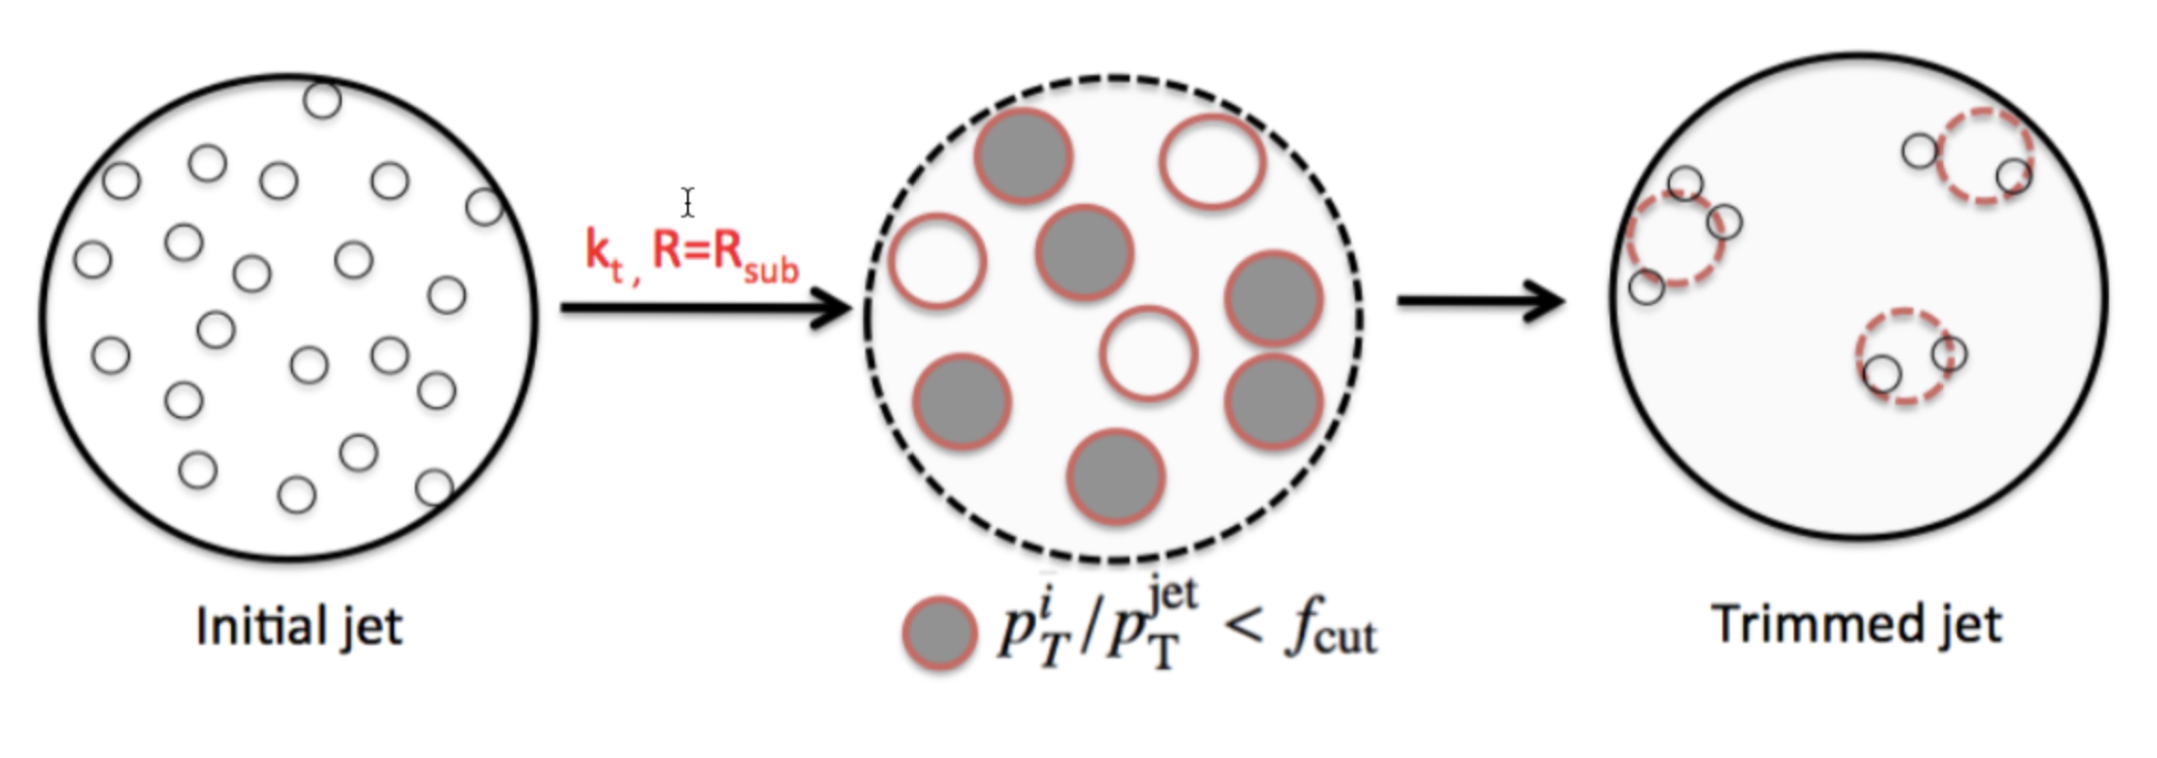
\includegraphics[width=0.9\linewidth]{jet_trimming}
\caption{Illustration of the trimming procedure, one of several grooming methods used to remove the contribution
of unassociated radiation to fat jet mass.}
\label{fig:jet_trimming}
\end{figure}

The values of $R_{sub}$ and $f_{cut}$ can be chosen to reduce pileup sensitivity and maximize jet mass resolution for the signal of interest.

The effect of different grooming techniques, including trimming, on jet mass resolution can be seen in figure~\ref{fig:jet_grooming_effect}.
For dijet events, high-mass jets are highly suppressed by grooming, which leads to a better signal-to-background ratio
for signals of hadronically decaying boosted objects with QCD dijet backgrounds.
For $t\bar{t}$ events, the top-mass peak is somewhat visible before grooming, although much wider than after grooming.
The $W$-mass peak, which is originally completely hidden due to unassociated radiation effects,
can be recovered with any of the grooming methods.

\begin{figure}[h!]
    \centering
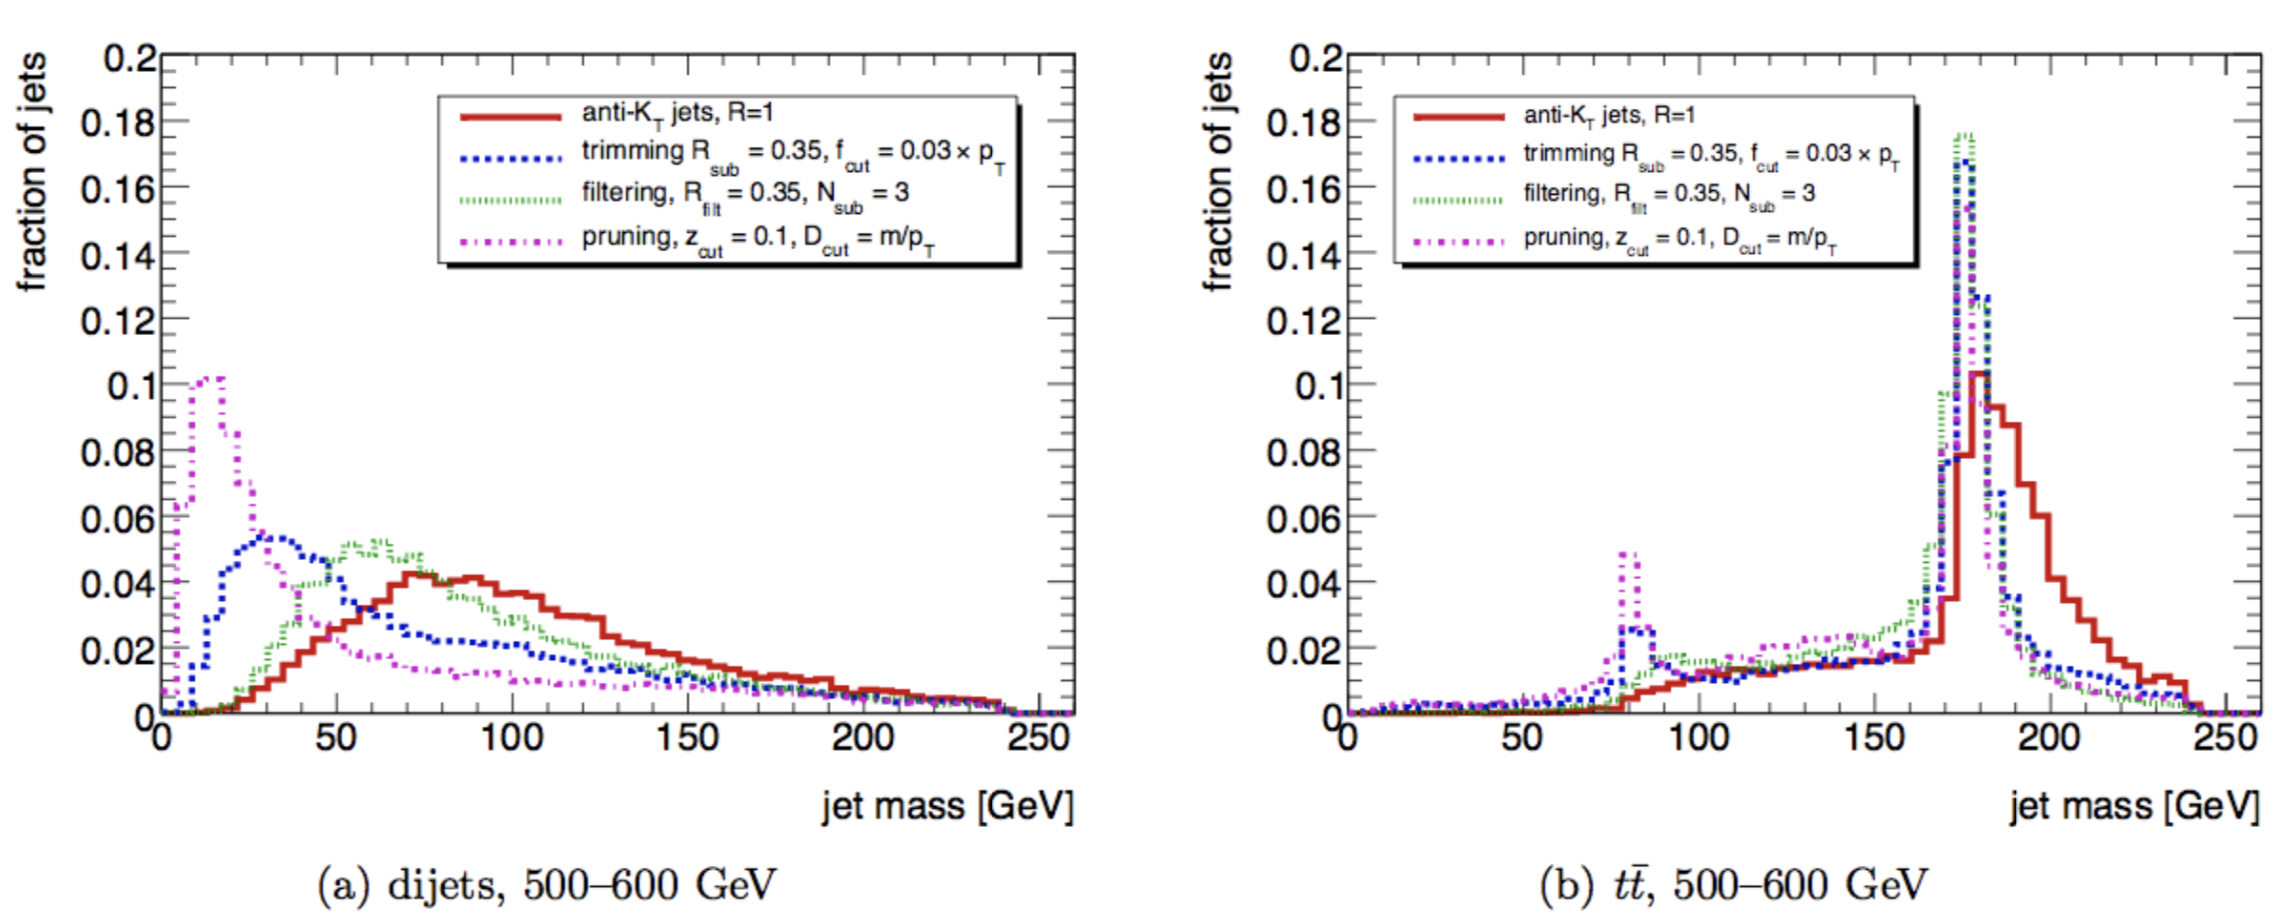
\includegraphics[width=0.9\linewidth]{jet_grooming_effect}
\caption{Measured jet mass distributions before and after grooming, for various grooming techniques.
Mass distributions are shown for both dijet events (left) and $t\bar{t}$ events (right).}
\label{fig:jet_grooming_effect}
\end{figure}

\section{Reconstruction in ATLAS}\label{sec:jet_reconstruction}
The goal of jet measurements in ATLAS is to capture and reconstruct both the energy and momentum of jets leaving the
collision point.
Calorimeter jets use clusters of calorimeter cell hits as inputs to the clustering algorithms outlined
in~\ref{sec:jet_clustering}.

\subsection{Topological cell clusters}\label{subsec:jet_topo_clusters}
\subsubsection{Clustering algorithm}\label{subsubsec:jet_topo_algo}
Topological cell clusters, or topo-clusters, are three-dimensional clusters of calorimeter cell energy measurements.
By clustering groups of calorimeter cells into topo-clusters, the number of inputs to the jet reconstruction algorithm
is reduced.
Topo-clustering also reduces calorimeter noise by rejecting cell signals not associated to other nearby significant
cell signals.\cite{jet-topo-cluster}
Topo-clusters serve as the main input to the jet clustering algorithms when reconstructing calorimeter jets in ATLAS .
The two sources of calorimeter cell noise are electronic noise and pileup.

The algorithm is based on the signal-to-noise ratio in each cell, $\zeta_{cell} = E_{cell}/\sigma_{cell}$.
There are three tunable parameters used in the algorithm, labeled $S$, $N$, and $P$, where $S > N \geq P$.

For purposes of the algorithm, a cell is considered to be a \textit{neighbor} of another cell if the two cells are
adjacent in the same layer, or if they are in adjacent layers and have any overlap.\cite{jet-topo-cluster}

The algorithm is as follows:
\begin{itemize}
    \item Label any cell with $\zeta_{cell}>S$ a seed cell.
    \item Collect all neighboring cells to a seed cell into a proto-cluster.
    \item If any cell in the proto-cluster has $\zeta_{cell}>N$, collect its neighbors into the proto-cluster.
    \item Repeat the previous step until the set of neighbors collected has $\zeta_{cell}<N$.
    \item Reject any cells with $\zeta_{cell}<P$.
\end{itemize}

At any time in the algorithm, if any cell with $\zeta_{cell}>N$ belongs two proto-clusters, then the two
proto-clusters are merged.\cite{jet-topo-cluster}

Once the algorithm terminates, the final set of topo-clusters are used as the inputs to the desired jet clustering
algorithm.

A result of this algorithm is that isolated cells with $\zeta_{cell} < N$ are rejected, which reduces that amount
of noise entering the jet clustering algorithm.
These cells are less likely to contain signal than cells with $\zeta_{cell}<N$ that neighbor cells with higher
signal-to-noise ratio.

This clustering algorithm does not guarantee that all the energy of a given particle in the jet will be captured by a single
topo-cluster, nor does it guarantee that a single topo-cluster only contains energy from a single particle.
So topo-clusters are not measurements of individual particles in the jet.

The three parameters $S$, $N$, and $P$ are tuned on test-beam data with known energy to maximize the measured energy
while minimizing the energy resolution\cite{jet-energy-measurement}.

Results of the test beam energy measurements with $180~GeV$and $20~GeV$ pions can be seen in~\ref{fig:jet_snp_tuning}.

\begin{figure}[h!]
    \centering
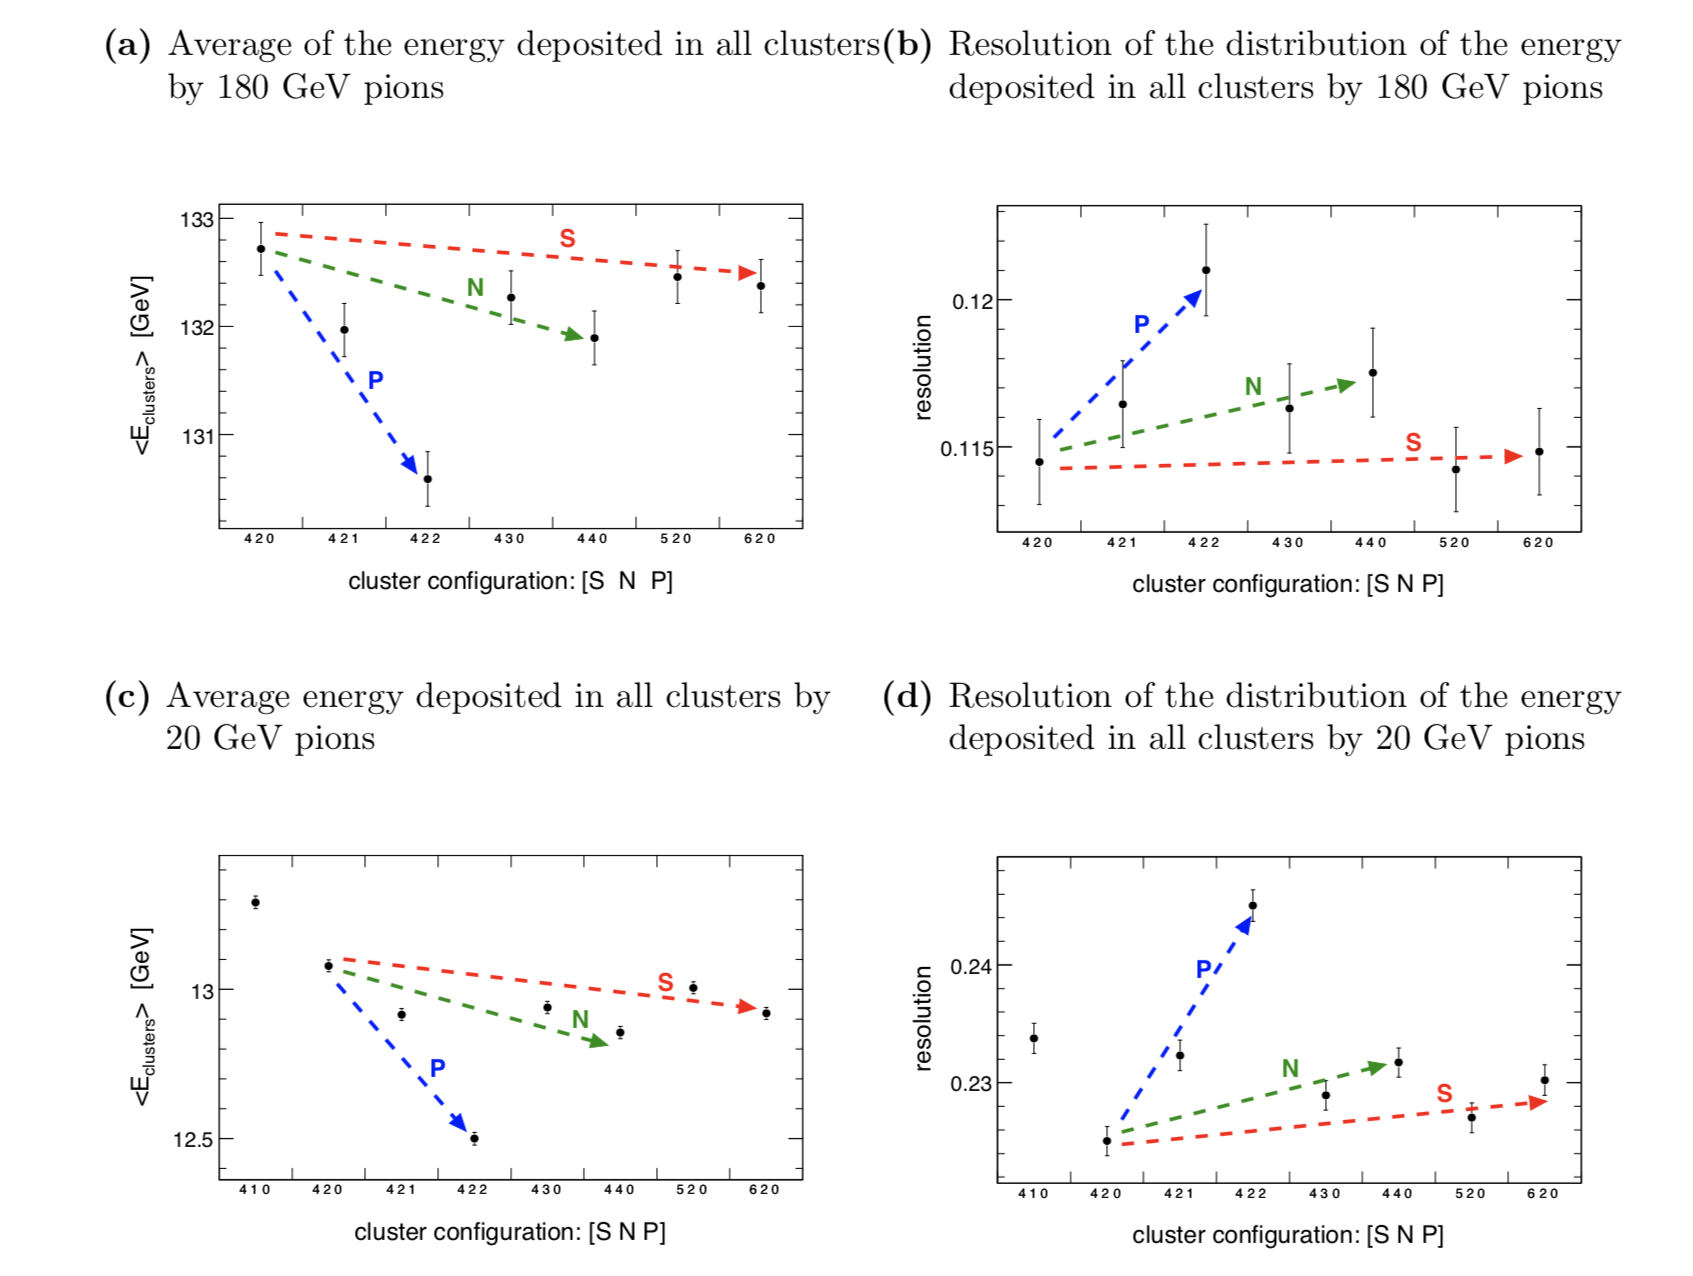
\includegraphics[width=0.9\linewidth]{jet_snp_tuning}
\caption{Average energy and energy resolution measured for $180~GeV$ and $20~GeV$ pions with different values of the
topo-clustering parameters $S$, $N$, and $P$.
The x-axis of each plot represents choices for all three parameters, and the y-axis indicates either the average
energy deposited in each cluster $<E_{clusters}>$ or the energy resolution $RMS/<E_{clusters}>$}
\label{fig:jet_snp_tuning}
\end{figure}\cite{jet-energy-measurement}

Based on these measurements, the default parameter values chosen for ATLAS topo-clustering are $S=4$, $N=2$, $P=0$.

\subsubsection{Topo-cluster moments}\label{subsubsec:jet_topo_moments}

\subsection{Calibration}\label{subsec:jet_calibration}
\subsection{Flavor Tagging}\label{subsec:jet_flavor_tagging}
\subsection{Simulation}\label{subsec:jet_full_vs_fast_sim}